\pdfvariable compresslevel=0
\documentclass[a4paper]{article}
\usepackage{pdfpages}
\usepackage{tikz}

\def\ExpectedResult{%
  \mbox{}\newpage
  \AddToShipoutPictureFG*{%
    \AtPageUpperLeft{%
      
\begin{tikzpicture}[overlay]
        \node [fill = green!20, below right]{\Huge Expected Result};
      \end{tikzpicture}}}}

\begin{document}

\def\bk#1{\texttt{booklet-#1.pdf}}
\Large
Difference between \bk{01} and \bk{05}:
\begin{description}
\item[\bk{01}] is set in global landscape mode,\break
  \verb!\documentclass[landscape]{...}!.
\item[\bk{05}] is set in global portrait mode, and only the included pages are
  set in landscape mode, \break
  \verb!\includpdf[landscape]{...}!.
\end{description}

\ExpectedResult
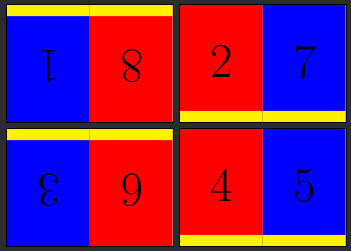
\includepdf[scale=0.5]{booklet/bk-01-01.png}

\includepdf[
  pages=-,
  nup=2x1, landscape,
  booklet,
]{booklet/normal-portrait.pdf}

\ExpectedResult
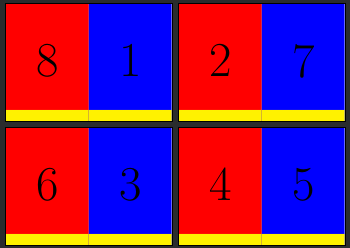
\includepdf[scale=0.5]{booklet/bk-01-02.png}

\includepdf[
  pages=-,
  nup=2x1, landscape,
  booklet,
  swap-flip-edge,
]{booklet/normal-portrait.pdf}

\ExpectedResult
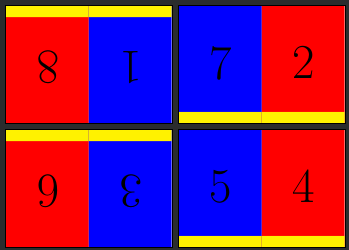
\includepdf[scale=0.5]{booklet/bk-01-03.png}

\includepdf[
  pages=-,
  nup=2x1, landscape,
  booklet*,
]{booklet/normal-portrait.pdf}

\ExpectedResult
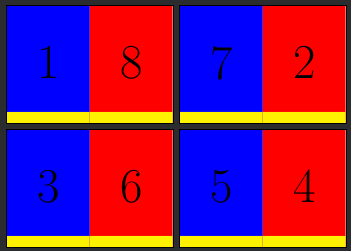
\includepdf[scale=0.5]{booklet/bk-01-04.png}

\includepdf[
  pages=-,
  nup=2x1, landscape,
  booklet*,
  swap-flip-edge,
]{booklet/normal-portrait.pdf}

\end{document}
